\chapter{Introdução} 
    \label{chap:Introducao}
    
Este capítulo tem como propósito contextualizar este Trabalho de Conclusão de Curso, conferindo definições sobre comércio eletrônico (em inglês,\textit{e-commerce}), comércio móvel (em inglês, \textit{m-commerce}), experiência de usuário e usabilidade. Usabilidade tem associação com experiência de usuário. Por isso, há necessidade de compreender ambos os conceitos desde a \nameref{con}. Na sequência, são apresentados: \nameref{jus}, \nameref{questao} e \nameref{ob}. Por fim, têm-se a \nameref{mono}.



\section{Contextualização} 
    \label{con}
    
O avanço e a disseminação das tecnologias móveis com acesso à internet, como \textit{smartphones} e \textit{tablets}, transformaram as expectativas das pessoas em relação aos seus dispositivos de comunicação. Nesse contexto, esses aparelhos tornaram-se essenciais no cotidiano das pessoas. Tal fato impulsionou a introdução de uma nova modalidade de comércio eletrônico, conhecida como comércio móvel (ou \textit{m-commerce}). Em contraste com o comércio eletrônico (ou \textit{e-commerce}) convencional, realizado principalmente em \textit{desktops} e \textit{laptops}, o \textit{m-commerce} tem se destacado globalmente como o método de vendas \textit{online} com o crescimento mais expressivo em termos de transações e faturamento. De acordo com \citeonline{LucasAlmeida}, esse método pode ultrapassar o comércio eletrônico tradicional nos próximos anos. 

Segundo \citeonline{SudianaChandra}, essa modalidade de compra, além de vantajosa para as empresas por permitir ampliar seu alcance a um custo mais baixo, também é vantajosa para o consumidor que consegue usufruir de comodidade no seu cotidiano. Os autores destacam que as pessoas tendem a abandonar os métodos tradicionais de compra, optando pelas compras feitas pela internet, o chamado comércio \textit{online}. Esse tipo de comércio abrange tanto a compra quanto a venda de produtos ou serviços, sendo ambas realizadas via sites e/ou aplicativos. Um fator muito importante para o crescimento desse setor foram as demandas ocorridas no período de pandemia da COVID-19, em 2020. Nesse período, houve maior necessidade quanto ao uso do comércio \textit{online}, visto que as pessoas se mantiveram em isolamento social. No Brasil, com base na pesquisa realizada pela \citeonline{RelatoriosEbit} em 2020, o número de pedidos \textit{online} saiu de uma média de 16\% nos primeiros três meses de 2020 para 57\% entre abril e junho do mesmo ano.

Para \citeonline{LucasAlmeida}, o \textit{m-commerce} traz consigo particularidades relacionadas aos processos comerciais, que se diferem quando acessados por dispositivos que proporcionam maior mobilidade. Uma dessas distinções diz respeito à plataforma de acesso disponível para transações comerciais. No comércio eletrônico tradicional, a interação ocorre exclusivamente por meio da navegação em sites; enquanto no \textit{m-commerce}, existem pelo menos duas principais fontes para efetivar tais processos, sendo: por meio de aplicativos, que são interfaces independentes desenvolvidas especificamente para acesso via dispositivos móveis; e também através de sites acessados por meio de navegadores presentes nesses dispositivos. Nesse último caso, ou seja, acesso via navegadores dos dispositivos, o \textit{design} responsivo tem se destacado recentemente como um tema revelante no âmbito do desenvolvimento web. Em linhas gerais, e com base em \citeonline{LucasAlmeida} o \textit{design} responsivo pode ser entendido como um processo de desenvolvimento que permite a adaptação de conteúdos e funcionalidades de uma página da Web às dimensões da tela de qualquer dispositivo, seja ele de formato fixo ou móvel.

Tendo em vista o cenário, no qual as pessoas estão utilizando cada vez mais sites e aplicativos pelo celular, fez-se presente a preocupação com a usabilidade dessas plataformas (no caso, sites e aplicativos de compra e venda \textit{online}). Segundo \citeonline{GunawanRicky}, a usabilidade nesse contexto impacta diretamente a experiência do usuário ao realizar uma compra ou uma venda. Adicionalmente, representa algo determinante para que o usuário continue navegando na plataforma, o que tende a ocorrer mais facilmente quando há adequadas usabilidade e experiência de usuário na plataforma. Dada a subjetividade do termo "adequada", no contexto desse trabalho, entende-se por "adequada" aquela usabilidade e/ou experiência de usuário orientada às boas práticas acordadas na literatura especializada, sejam livros \cite{AtomicDesignFrost}, materiais acadêmicos \cite{HeuristicasNielsen} ou ainda materiais divulgados por empresas reconhecidas em \textit{UI/UX Design (User Interface/User Experience Design)} \cite{MaterialDesign3}. Um maior detalhamento sobre essas práticas será conferido no \hyperref[chap:ReferencialTeorico]{Capítulo 2 - Referencial Teórico}.

Tendo em mente que uma das principais intenções das plataformas disponíveis \textit{online} é atrair um quantitativo maior de clientes que desejam comprar e vender, há demanda de facilitadores que promovam a comunicação clara e simples entre humanos e essas plataformas. Logo para uma empresa manter a excelência no atendimento ao cliente e agregar valor a ele é oferecendo uma plataforma bem projetada. Garantir o sucesso e a conclusão das transações de compra e venda não é mais suficiente. Descobriu-se que um site bem projetado poderia proporcionar uma experiência positiva ao usuário. O \textit{design} em um site ou em qualquer outro meio de exibição fornecido ao usuário desempenha um papel muito importante no sucesso do comércio eletrônico. Uma das coisas que desempenha o papel mais importante na criação de uma boa imagem é sempre tornar mais fácil fornecer informações aos usuários para que eles possam ver produtos e informações claramente \cite{SudianaChandra}.

É fundamental diferenciar o que são usabilidade e experiência do usuário. Para \citeonline{NNGroupUI} e \citeonline{UsabilidadeJoao}, a usabilidade representa um critério de qualidade que avalia a facilidade de utilização das interfaces destinadas aos usuários. Dentre alguns aspectos importantes a serem analisados, destacam-se cinco atributos: Aprendizagem, Eficácia, Memorização, Erros e Satisfação. Dessa forma, para um sistema existir de forma agradável aos usuários, é desejável que esses cinco critérios sejam considerados no \textit{design} desse sistema. Um sistema de fácil aprendizagem tende a permitir que seus usuários realizem suas atividades de forma rápida e eficaz. Adicionalmente, a memorização do processo tende a ocorrer de forma natural, possibilitando inclusive que o usuário seja capaz de perceber erros e se recuperar dos mesmos, e culminando em uma maior satisfação do usuário, que conseguiu seguir o fluxo desejado no sistema.

A experiência do usuário é um conceito mais abrangente, comparativamente ao conceito de usabilidade. No caso da experiência do usuário, têm-se todos os elementos da interação do usuário final com os serviços, produtos e a entidade empresarial em si, de acordo com a \citeonline{ISO924210}. Além disso, é influenciada pelas experiências anteriores, atitudes, habilidades, padrões de comportamento e características individuais do usuário.

O principal critério para garantir uma experiência de usuário adequada, segundo \citeonline{NNGroupUX}, é satisfazer precisamente as demandas do usuário, mitigando qualquer forma de desconforto. Adicionalmente, cabe buscar simplicidade, sem desvalorizar o que é fornecido, resultando na criação de produtos que oferecem satisfação ao serem adquiridos e utilizados.

Tanto a usabilidade quanto a experiência de usuário são critérios de qualidade de igual importância. Quando combinados, esses critérios determinam a eficácia de algo. Nesse contexto,  os autores \citeonline{NNGroupUX} mencionam que não basta algo ser fácil, se esse algo não atende ao que se deseja. Da mesma forma, não é desejado um sistema que, em teoria, realiza o que se pretende; porém, devido à complexidade da interface, torna-se impraticável realizar tais ações pretendidas.

Diante do exposto, é recomendado que se atente à usabilidade e à experiência de usuário quando projetados sistemas no domínio de comércio eletrônico e/ou comércio móvel, uma vez que os usuários desses sistemas precisam se sentir confortáveis, satisfeitos, ao interagirem com os sistemas. Ao tratar a usabilidade, o sistema tende a proporcionar ao usuário uma sensação de independência, aumentando a confiança desse usuário ao realizar suas atividades e, consequentemente, facilitando o uso e o aprendizado. Tais sucessos tendem a impactar positivamente a experiência de usuário.



\section{Justificativa} 
    \label{jus}
    
De acordo com a pesquisa da Agência \citeonline{ConversionDocs}, realizada no período compreendido entre janeiro e outubro de 2023, a média de acessos do \textit{e-commerce} no Brasil foi de 2,51 bilhões por mês. O melhor momento do ano foi em julho, com 2,61 bi de visitas registradas. Tendo em vista esse cenário, e compreendendo que essa demanda está muito associada ao comércio móvel (ou seja, ao domínio de interesse do presente trabalho), aprimorar a experiência do usuário pode ter um impacto positivo nas intenções dos usuários enquanto compram e vendem produtos e serviços. Segundo \citeonline{GunawanRicky}, essa experiência mais aprimorada pode ser conquistada quando os usuários se deparam e interagem com uma interface de fácil uso, bem projetada. Ainda com base nos autores, tem-se que o \textit{design} orientado a interfaces de fácil uso proporciona conforto ao usuário, incentivando o uso contínuo dessa interface e, consequentemente, aprimorando a experiencia do usuário até mesmo em futuros desenvolvimentos de \textit{software} similares.

Segundo os resultados da pesquisa dos autores \citeonline{SudianaChandra}, os principais fatores do \textit{design} que impactam a experiência do usuário são \textit{design} visual, a qualidade das informações, a facilidade de navegação, a usabilidade e o desempenho em termos de velocidade e tempo de carregamento. Esses elementos têm sido amplamente propostos e aplicados na prática por diversas empresas. Sendo assim, o objetivo principal de uma empresa ao desenvolver uma plataforma de comercio eletrônico e comércio móvel é atrair um grande número de visitantes, para assim torná-los clientes, impulsionando o aumento das vendas e, consequentemente, dos lucros. Dessa forma, é recomendado que a empresa priorize a experiência do usuário.

Considerando dados mais recentes de uma pesquisa da \cite{ConversionDocs}, realizada em Fevereiro de 2024 referente ao mês de Janeiro de 2024, mostrou um crescimento de 3,6\% no movimento do comércio eletrônico brasileiro. É possível concluir que investir em uma melhor usabilidade levando assim a uma melhor experiência para o cliente é vantajoso, como mostra a figura \label{fig04}. A pesquisa analisou o tráfego dos 2000 maiores sites do Brasil, dividindo em um total de 18 categorias sendo analisados no mínimo de 20 sites para cada. Os dados são referentes a acessos em território brasileiro verificando dispositivos \textit{mobile, desktop} e aplicativos \textit{Android}.

\begin{figure}[ht]
    \centering
    \caption{Crescimento de Dez/23 para Jan/23 do movimento do comércio eletrônico no Brasil}
    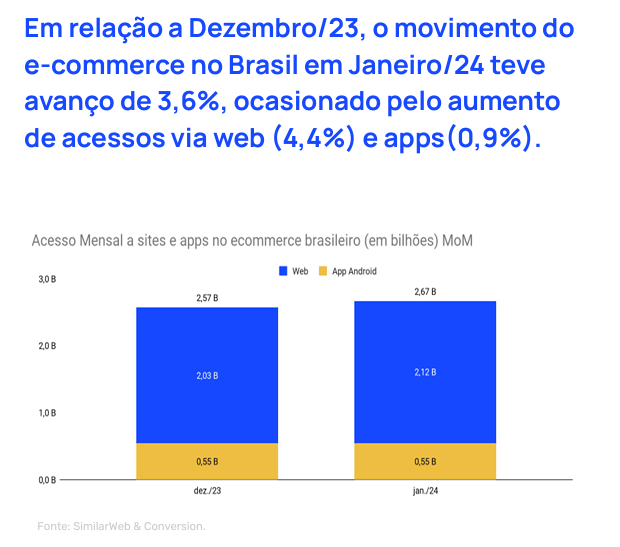
\includegraphics[keepaspectratio=true,scale=0.6]{figuras/cap02ConversionJan2024.png}
    \legend{Fonte: \textit{SimilarWeb e Conversion}, Relatório E-commerce de Jan/24}
    \label{fig04}
\end{figure}

Considerando o exposto, este trabalho visa identificar quais são as principais dificuldades encontradas pelos usuários ao utilizarem plataformas de comércio eletrônico móvel mais populares. Entende-se por plataformas populares as mais acessadas e conhecidas no domínio de comércio eletrônico móvel. Tendo em mente o âmbito Brasil, há necessidade de realizar um levantamento para estabelecer essas principais plataformas, sendo esse levantamento também realizado ao longo do presente estudo. Dentre as plataformas encontradas, será selecionada uma como exemplo, para facilitar a condução desse estudo como um todo.

Como intuito adicional, ao identificar as principais dificuldades encontradas pelos usuários, será realizada uma associação entre essas dificuldades e as principais técnicas/práticas de usabilidade que impactam positivamente na experiência de usuário e mitigam tais dificuldades. Com essa associação estabelecida, serão aplicadas melhorias na plataforma popular escolhida como exemplo, principalmente na interface, usando como base protótipos de alta fidelidade. Em meio a outros insumos, o estudo proposto, portanto, tende a oferecer: (i) o levantamento das plataformas mais populares de comércio eletrônico móvel; (ii) o levantamento das principais dificuldades encontradas pelos usuários ao interagirem com uma dessas plataformas selecionada como exemplo; (iii) a associação entre essas dificuldades e as técnicas/práticas de usabilidade, disponíveis na literatura especializada, e orientadas à experiência de usuário, que mitigam tais dificuldades, e (iv) aplicação dessas técnicas/praticas na plataforma exemplo, via protótipos de alta fidelidade.



\section{Questão de Pesquisa} 
    \label{questao}
    
O presente trabalho pretende responder a seguinte questão de pesquisa: Como prover melhorias nas plataformas de comércio eletrônico móvel tendo como base técnicas/práticas de usabilidade orientadas à experiência de usuário?

Percebe-se, com a questão apresentada, que o estudo proposto está compreendido na grande área Engenharia de Software, mais especificamente na subárea de Interação Humano-Computador, com foco no domínio de comércio eletrônico móvel e nos critérios qualitativos usabilidade e experiência de usuário. Há necessidade de explorar, adicionalmente: técnicas de elicitação e validação para os inerentes levantamentos a serem realizados, provavelmente a técnica de questionário, e técnicas de design, mais precisamente a prototipação para elaboração das interfaces melhoradas com a aplicação das técnicas/práticas de usabilidade.



\section{Objetivos} 
    \label{ob}
    
Seguem os objetivos, sendo os mesmos de cunho geral e específicos.

\subsection{Objetivo Geral}
O objetivo geral deste TCC é o estudo sobre experiência de usuário no domínio de comércio eletrônico móvel.

No intuito de cumprir com o objetivo geral, e dada a abrangência do mesmo, são especificados alguns objetivos específicos, conforme seguem:

\subsection{Objetivos Específicos}
	\begin{itemize}
		\item Levantamento teórico sobre o comércio eletrônico móvel no Brasil;
        \item Pesquisa na literatura acadêmica referente aos conceitos de usabilidade e experiência de usuário;
        \item Identificação das principais dificuldades encontradas pelos usuários ao interagirem com plataformas de comércio eletrônico móvel;
        \item Associação entre as dificuldades identificadas no objetivo anterior e as principais técnicas/práticas de usabilidade orientadas à experiência de usuário;
        \item Aplicação de melhorias - prototipagem - em uma plataforma de comércio eletrônico móvel, com base na associação obtida com o cumprimento do objetivo específico anterior.
	\end{itemize} 

Adicionalmente, cabe ressaltar que haverá documentação do estudo como um todo, revelando sobre os questionários realizados bem como demais insumos inerentes ao estudo proposto.



\section{Organização da Monografia} 
    \label{mono}
    
Essa monografia está organizada em capítulos, sendo o presente capítulo introdutório, e os demais:

\hyperref[chap:ReferencialTeorico]{Capítulo 2 - Referencial Teórico}: capítulo dedicado aos principais conceitos que fundamentam o estudo proposto, com destaque para Comércio Eletrônico Móvel, Usabilidade e Experiência de Usuário;

\hyperref[chap:ReferencialTecnologico]{Capítulo 3 - Referencial Tecnológico}: capítulo focado nas principais ferramentas e tecnologias usadas para viabilizar o trabalho;

\hyperref[chap:Metodologia]{Capítulo 4 - Metodologia}: capítulo que esclarece sobre a metodologia para realização do trabalho em termos investigativo, desenvolvimento e análise de resultados;

\hyperref[chap:Proposta]{Capítulo 5 - Proposta}: capítulo que procura apresentar detalhes complementares sobre a presente proposta, e

\hyperref[chap:ConsideracoesFinais]{Capítulo 6 - Considerações Finais}: capítulo que resgata os principais pontos tratados na proposta, procurando apresentar o status atual do trabalho.